\documentclass[aspectratio=169]{beamer}
\usetheme{Madrid}
\usecolortheme{default}
\usepackage{graphicx}
\usepackage{booktabs}
\usepackage{hyperref}
\title{Predicting Steel Quality from Production Measurements}
\subtitle{Applied Machine \& Deep Learning (190.015)\\Project P1}
\author{}
\institute{Winter Semester 2026/27}
\date{}

\begin{document}

\begin{frame}
  \titlepage
\end{frame}

\begin{frame}{Task and dataset}
  \begin{itemize}
    \item Predict the continuous steel-quality target \texttt{output}.
    \item 21 process measurements are supplied as \texttt{input1}--\texttt{input21}.
    \item Training file: 7,642 rows; provided test file: 3,337 rows.
    \item Both files contain 22 numeric columns; the recorded audit found no missing values or duplicate rows.
    \item Physical units and meanings of the columns are not provided.
  \end{itemize}
  \vspace{0.5em}
  \small Motivation: test whether production measurements contain useful signal for predicting the quality factor.
\end{frame}

\begin{frame}{Data exploration}
  \begin{columns}[T]
    \column{0.68\textwidth}
      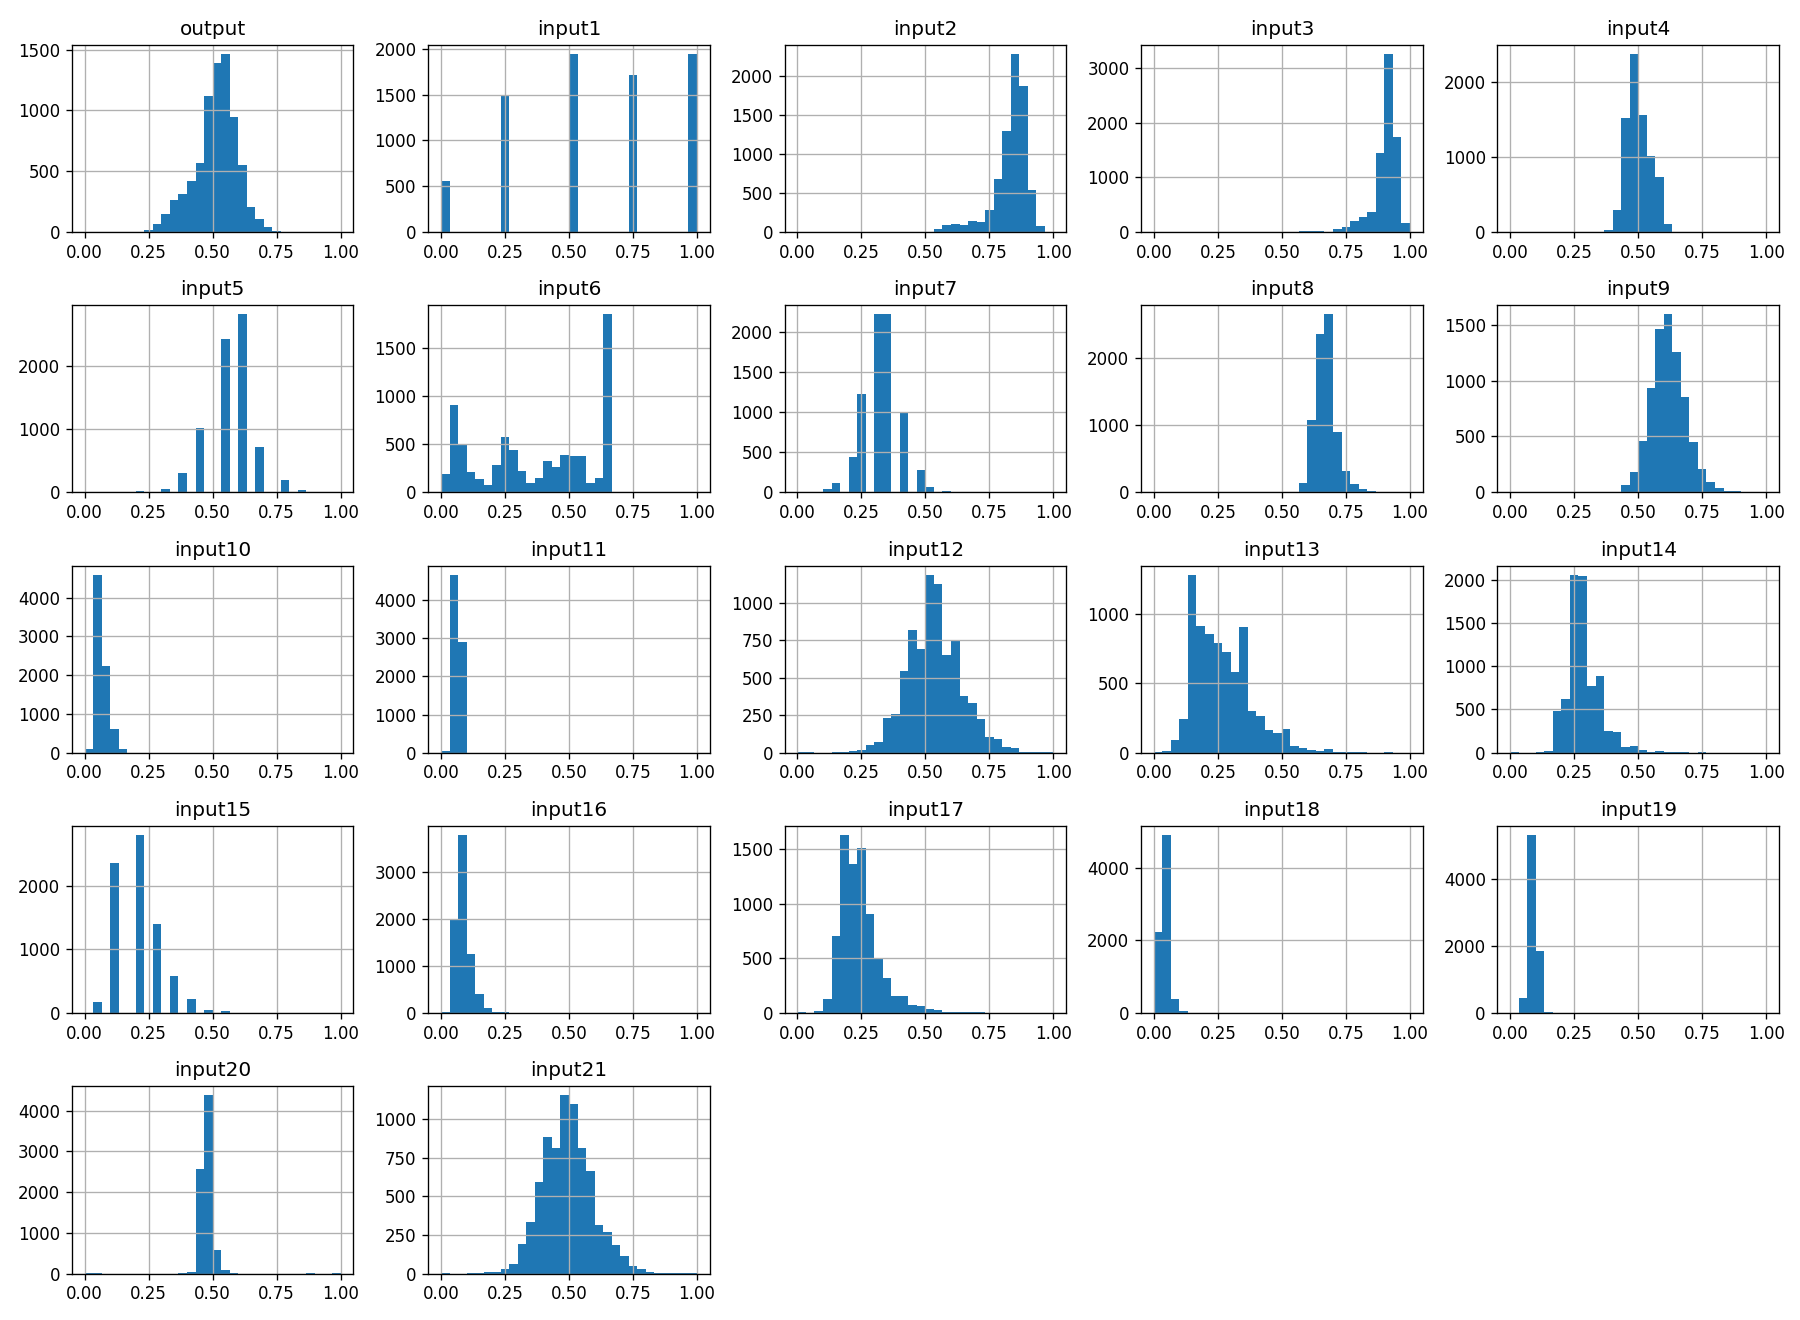
\includegraphics[width=\linewidth]{../results/figures/histograms.png}
    \column{0.30\textwidth}
      \small
      Training data were checked for duplicates, missing values and column types.

      \vspace{0.8em}
      Inputs are already normalized in the supplied files. No physical interpretation is assigned to anonymized columns.
  \end{columns}
\end{frame}

\begin{frame}{Preprocessing and evaluation design}
  \begin{itemize}
    \item Remove exact duplicates; drop rows without a target.
    \item Split training file into 80\% train and 20\% validation (seed 42); retain the supplied test file.
    \item Clip numeric outliers to $Q_1-3\,IQR$ and $Q_3+3\,IQR$ fences calculated on the training partition.
    \item Fit median imputation and standardization in the numeric model pipeline; one-hot encode categorical data if present.
    \item Compare with shuffled five-fold CV; report mean $\pm$ standard deviation across folds.
  \end{itemize}
  \vspace{0.5em}
  \footnotesize Caveat: outlier fences are currently estimated before CV folds are created, so held-out fold features contribute to those fence estimates.
\end{frame}

\begin{frame}{Compared regression models}
  \begin{table}
    \centering
    \begin{tabular}{lll}
      \toprule
      Model & Family & Main setting \\
      \midrule
      Ridge & Linear, $L_2$ regularized & $\alpha=1$ \\
      Random forest & Tree ensemble & 200 trees; leaf size 2 \\
      SVR & Kernel regression & $C=1$; $\epsilon=0.02$ \\
      \bottomrule
    \end{tabular}
  \end{table}
  \begin{itemize}
    \item RMSE and MAE: lower is better.
    \item $R^2$: higher is better; negative means worse than predicting the evaluation-set mean.
    \item No hyperparameter search was performed.
  \end{itemize}
\end{frame}

\begin{frame}{Five-fold cross-validation}
  \begin{columns}[T]
    \column{0.61\textwidth}
      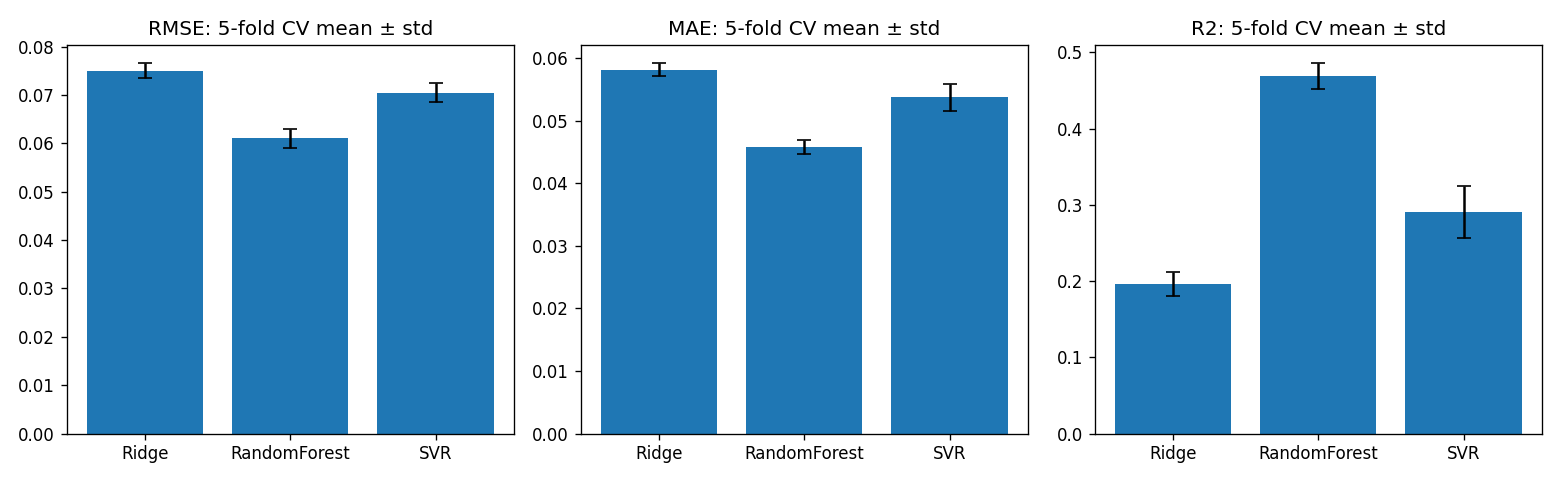
\includegraphics[width=\linewidth]{../results/figures/model_comparison.png}
    \column{0.38\textwidth}
      \small
      \begin{tabular}{lrr}
        \toprule
        Model & RMSE & $R^2$ \\
        \midrule
        Ridge & $0.0751\pm0.0015$ & $0.196\pm0.016$ \\
        Random forest & $\mathbf{0.0610\pm0.0019}$ & $\mathbf{0.469\pm0.017}$ \\
        SVR & $0.0705\pm0.0020$ & $0.291\pm0.034$ \\
        \bottomrule
      \end{tabular}

      \vspace{0.8em}
      Random forest has the best mean RMSE, MAE and $R^2$ across the five folds.
  \end{columns}
\end{frame}

\begin{frame}{Validation versus supplied test}
  \begin{table}
    \centering
    \begin{tabular}{lrrrr}
      \toprule
      & \multicolumn{2}{c}{Validation} & \multicolumn{2}{c}{Provided test} \\
      Model & RMSE & $R^2$ & RMSE & $R^2$ \\
      \midrule
      Ridge & 0.0769 & 0.110 & 0.1609 & -1.895 \\
      Random forest & \textbf{0.0617} & \textbf{0.428} & 0.1717 & -2.297 \\
      SVR & 0.0718 & 0.224 & \textbf{0.1405} & \textbf{-1.206} \\
      \bottomrule
    \end{tabular}
  \end{table}
  \begin{itemize}
    \item Random forest leads on the internal validation split.
    \item All three models have negative $R^2$ on the supplied test file.
    \item Holdout metrics are single evaluations, not repeated-run means or standard deviations.
  \end{itemize}
\end{frame}

\begin{frame}{Generalization diagnostic}
  \begin{columns}[T]
    \column{0.62\textwidth}
      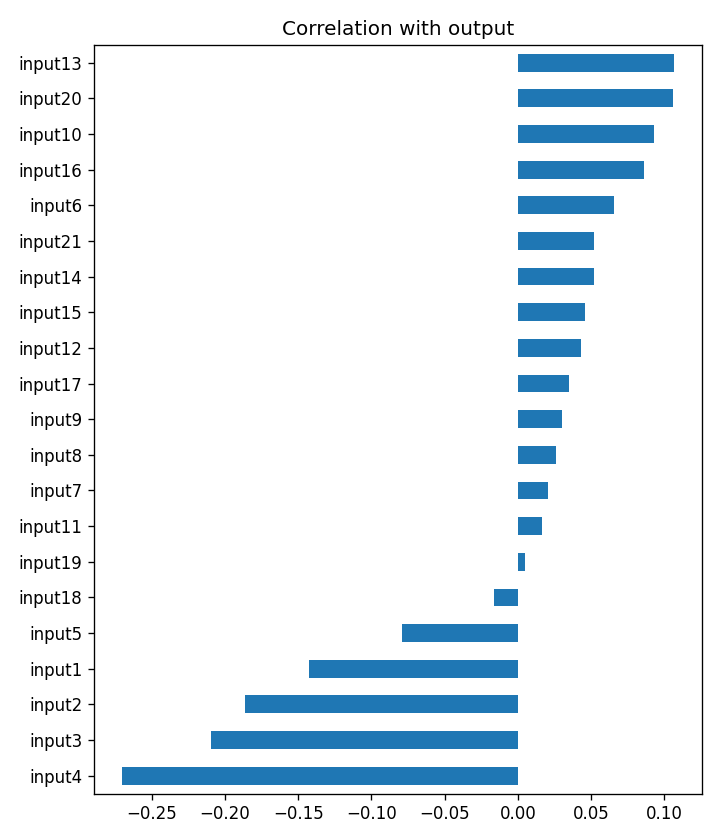
\includegraphics[width=\linewidth]{../results/figures/correlation_with_output.png}
    \column{0.36\textwidth}
      \small
      Repository exploration notes that each file spans 0--1 column-wise, while some feature means differ (e.g., \texttt{input3}: train 0.90, test 0.36).

      \vspace{0.8em}
      This suggests a train--test difference, but does not prove its cause. Separate scaling or distribution shift is a hypothesis to verify.
  \end{columns}
\end{frame}

\begin{frame}{Conclusion and next steps}
  \begin{itemize}
    \item Random forest is the strongest of the three models in CV and validation.
    \item The negative test $R^2$ values mean none is ready for use on the supplied test data.
    \item Confirm the test file's provenance and normalization with the course.
    \item Re-estimate outlier fences inside each CV training fold and rerun the evaluation.
    \item Only then consider tuning models or drawing production conclusions.
  \end{itemize}
\end{frame}

\begin{frame}{Selected references}
  \footnotesize
  \begin{thebibliography}{9}
    \bibitem{millner2023}
    G. Millner et al., ``Machine learning mechanical properties of steel sheets from an industrial production route,'' \emph{Materialia}, 30, 101810, 2023.
    \href{https://doi.org/10.1016/j.mtla.2023.101810}{doi:10.1016/j.mtla.2023.101810}.

    \bibitem{breiman2001}
    L. Breiman, ``Random forests,'' \emph{Machine Learning}, 45, 5--32, 2001.
    \href{https://doi.org/10.1023/A:1010933404324}{doi:10.1023/A:1010933404324}.

    \bibitem{cortes1995}
    C. Cortes and V. Vapnik, ``Support-vector networks,'' \emph{Machine Learning}, 20, 273--297, 1995.
    \href{https://doi.org/10.1007/BF00994018}{doi:10.1007/BF00994018}.
  \end{thebibliography}
\end{frame}

\end{document}
